\subsubsection{Deployment}
\label{subsec:kubernetes:deployment}
Deployments beschreiben deklarativ ein Template für Pods \cite{kubernetesDeployments}. 

Das manuelle Aktualisieren von Pods kann mühselig und fehlerbehaftet sein. Bei Softwareänderungen und damit dem
Bereitstellen neuer Container Images muss sichergestellt sein, dass alte Pods erst gelöscht werden, wenn die neue Version
lauffähig ist. Falls dies nicht der Fall ist, kann dies zu einer erhöhten Ausfallzeit führen \cite{Marko2018}.
Um diese Ausfallzeit zu minimieren, verwendet ein Deployment standardmäßig eine \emph{Rolling Update} Strategie.
Hierbei werden bei Änderungen des Templates alte Pods nach und nach entfernt und zeitgleich neue Pods hinzugefügt.
Dadurch wird sichergestellt, dass die Anwendung während des gesamten Prozesses verfügbar bleibt und die Kapazität zur Bearbeitung
von Anfragen nicht nachlässt \cite{Marko2018}.
Zur Veranschaulichung wird diese Strategie in \ref{fig:kubernetes_rolling_update} dargestellt.

\begin{figure}
  \centering
  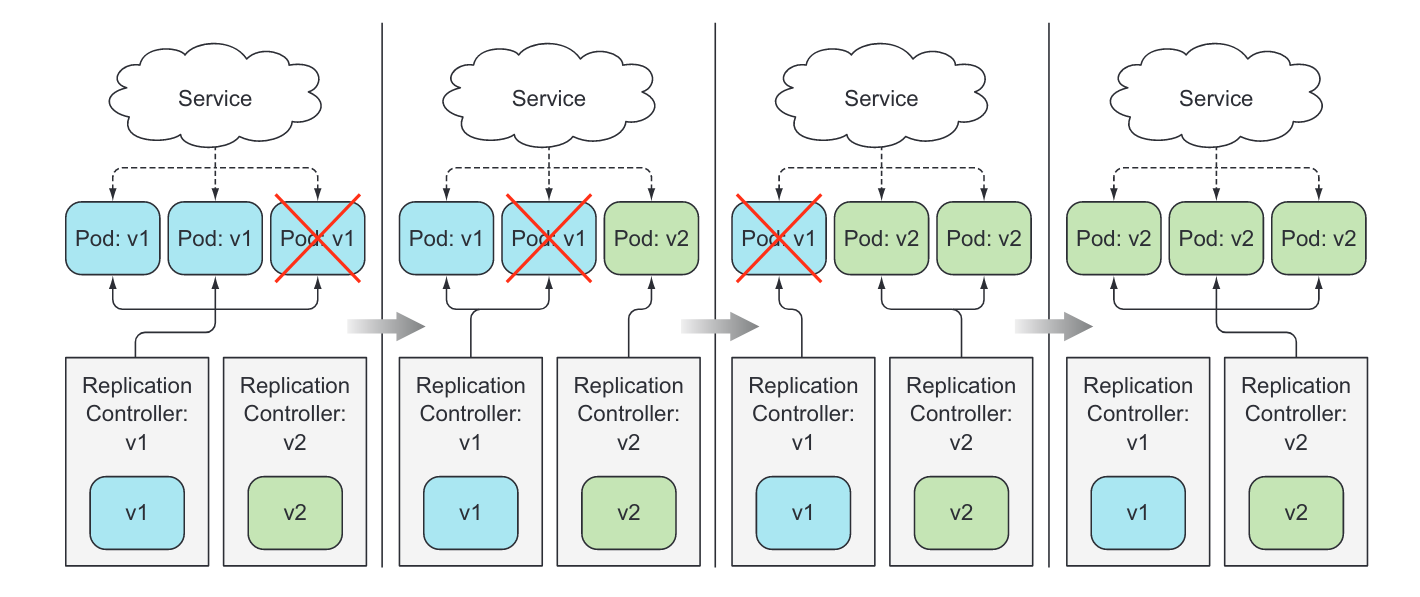
\includegraphics[width=\textwidth]{gfx/chapters/2_grundlagen/deployment_rollout.png}
  \caption{Rolling Update Strategie eines Deployments}
  \label{fig:kubernetes_rolling_update}
  \source{\cite{kubernetesRollingUpdate}}
\end{figure}

Die beiden meistgenutzten Tätigkeiten eines Deployments sind das Ändern sowie Skalieren von Anwendungen \cite{Burns2019}.
Zudem bieten Deployments neben automatischer Aktualisierung von Pods die Möglichkeit des Zurückrollens von Änderungen \cite{kubernetesDeployments}.
